\documentclass[xcolor=dvipsnames,compress]{beamer}
\usepackage{CJK}
\usepackage[italian]{babel}
\usepackage[latin1]{inputenc}
\usepackage[T1]{fontenc}

%\definecolor{necstgreen}{rgb}{0.137,0.466,0.741}
%\definecolor{necstgreen}{RGB}{240,40,40}

%\definecolor{necstgreen}{RGB}{187,216,113}
\definecolor{necstgreen}{RGB}{171,216,80}
\definecolor{necstgreen2}{RGB}{141,193,0}
\definecolor{necstgray}{RGB}{20,20,20}

\usetheme{Madrid}
\useoutertheme[subsection=false]{miniframes}
\useinnertheme{rectangles}
\usecolortheme[named=necstgreen2]{structure}
\setbeamercolor*{palette primary}{use=structure,fg=black,bg=necstgreen}
%\setbeamertemplate{items}[ball,bg=necstgreen] 
%\setbeamertemplate{blocks}[rectangles][shadow=false] 
\setbeamertemplate{items}[circle]

\defbeamertemplate*{title page}{customized}[1][]
{
  \vbox{}
  \vfill
  \begin{centering}
    \begin{beamercolorbox}[sep=8pt,center,rounded=true,shadow=true]{title}
      \usebeamerfont{title}\inserttitle\par%
      \ifx\insertsubtitle\@empty%
      \else%
        \vskip0.25em%
        {\usebeamerfont{subtitle}\usebeamercolor[fg]{subtitle}\insertsubtitle\par}%
      \fi%     
    \end{beamercolorbox}%
    \vskip1em
    \vfill
    \par
    \begin{beamercolorbox}[sep=8pt,center,#1]{author}
      \usebeamerfont{author}\textbf{Middleware Project Presentation of} \\ \insertauthor
    \end{beamercolorbox}
    \begin{beamercolorbox}[sep=8pt,center,#1]{institute}
      \usebeamerfont{institute}\insertinstitute
    \end{beamercolorbox}
    \begin{beamercolorbox}[sep=8pt,center,#1]{date}
      \usebeamerfont{date}\insertdate
    \end{beamercolorbox}\vskip0.5em
    {\usebeamercolor[fg]{titlegraphic}\inserttitlegraphic\par}
  \end{centering}
}


\AtBeginSection[]{
\begin{frame}
	\begin{center}
		\begin{beamercolorbox}[sep=8pt,center,rounded=true,shadow=true]{part title}
        \usebeamerfont{part title}\insertsection
     \end{beamercolorbox}
\end{center}
\end{frame}
}

\setbeamercolor{section in head/foot}{fg=white, bg=necstgray}
\setbeamercolor{author in head/foot}{fg=black, bg=necstgreen}
\setbeamercolor{logo in head/foot}{fg=white, bg=necstgray}
\setbeamercolor{page number in head/foot}{fg=black, bg=necstgreen}

\setbeamertemplate{footline}
{
  \leavevmode%
  \hbox{%
  \begin{beamercolorbox}[wd=.10\paperwidth,ht=2.25ex,dp=1ex,center]{logo in head/foot}%
    \usebeamerfont{logo in head/foot}NECSTLab
  \end{beamercolorbox}%
  \begin{beamercolorbox}[wd=.20\paperwidth,ht=2.25ex,dp=1ex,center]{author in head/foot}%
    \usebeamerfont{author in head/foot}\insertshortauthor
  \end{beamercolorbox}%
  \begin{beamercolorbox}[wd=.65\paperwidth,ht=2.25ex,dp=1ex,center]{title in head/foot}%
    \usebeamerfont{title in head/foot}\insertshorttitle
  \end{beamercolorbox}}%
  \begin{beamercolorbox}[wd=.05\paperwidth,ht=2.25ex,dp=1ex,center]{page number in head/foot}%
    \usebeamerfont{page number in head/foot}\insertframenumber
  \end{beamercolorbox}%
  \vskip0pt%
}


\begin{document}
\setbeamertemplate{navigation symbols}{}

\title[Distributed Tic Tac Toe]{Tic Tac Toe Application\\ using JMS }
		
\author[A. Mambretti]{Andrea Mambretti, \small{matr. 783286}\\~\\ \textbf{Professor:} Prof. Gianpaolo Cugola\\ \textbf{Assistant:} Ing. Alessandro Sivieri\vspace{0.3cm}}

\institute{\hfill\begin{columns}\begin{column}{0.20\columnwidth}\hfill
\includegraphics[width=0.8\columnwidth]{img/PoliMI.eps}\end{column} \begin{column}{0.45\columnwidth}\centering Politecnico di Milano\\Scuola di Ingegneria Industriale e dell'Informazione\\Corso di Laurea Magistrale in Ingegneria Informatica\end{column}\begin{column}{0.2\columnwidth}\hfill
\includegraphics[scale=0.8]{img/necst-official-logo-white}\end{column}\end{columns}}

\date{}

\frame[plain]{\vspace{1.1cm}\titlepage}

\section[Infrustructure]{Overview}
\subsection{}
\frame{\frametitle{Basic schema}
\begin{figure}
\centering
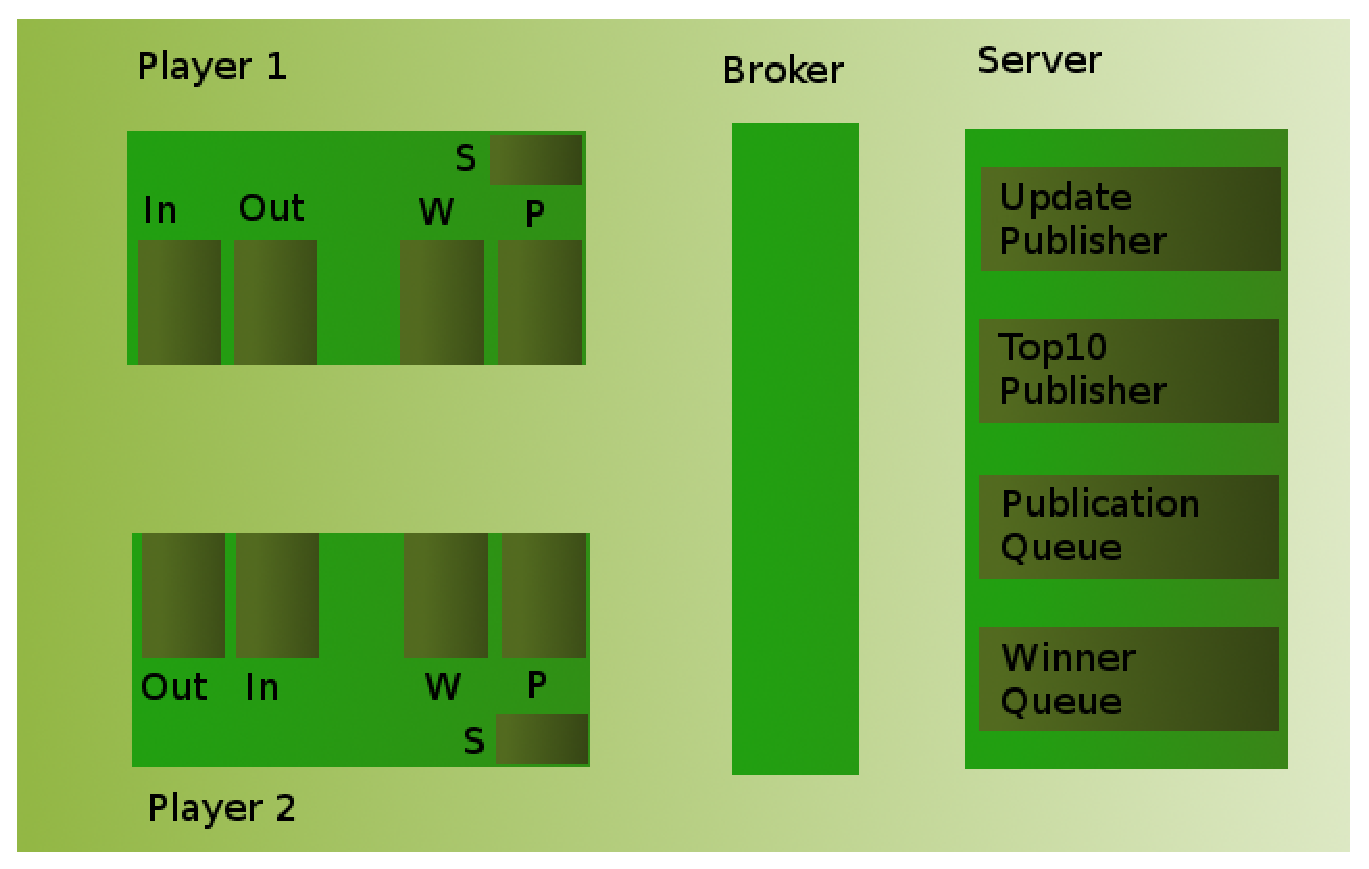
\includegraphics[scale=0.4]{img/schema_tictactoe.eps}
\end{figure}
}

\frame{\frametitle{Demo schema}
\begin{figure}
\centering
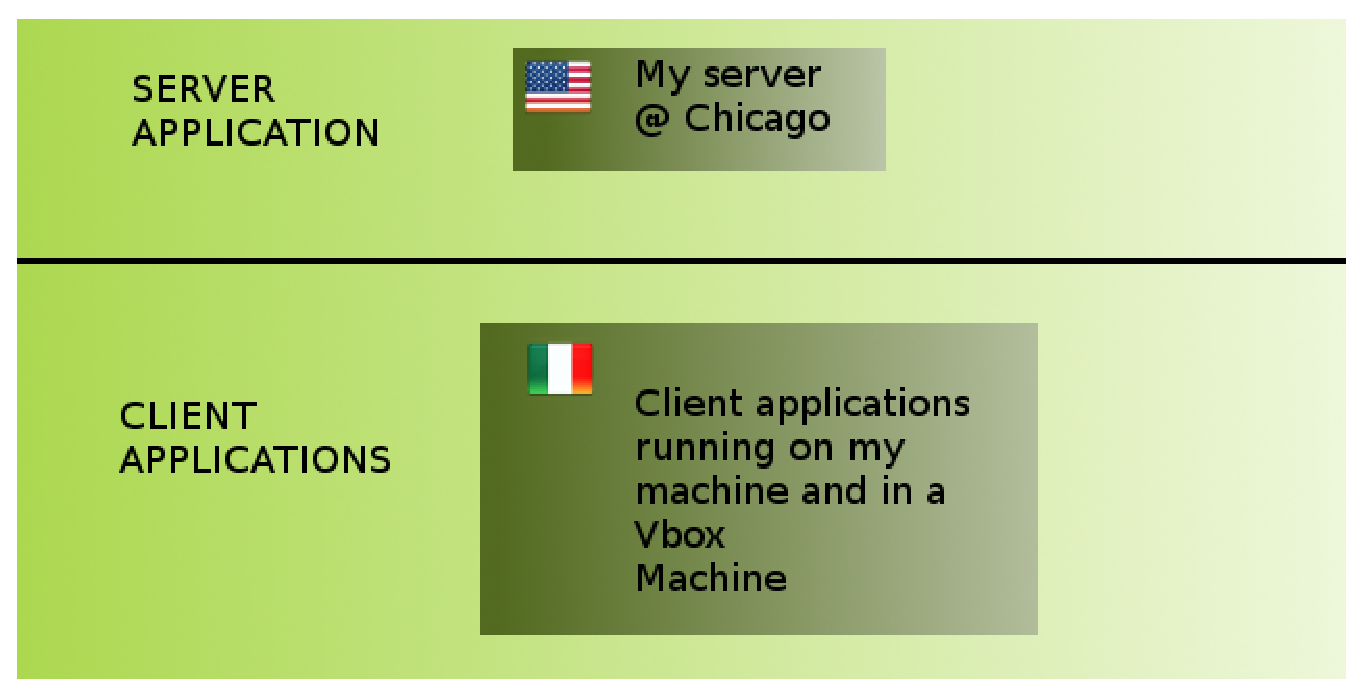
\includegraphics[scale=0.4]{img/demo_tictactoe.eps}
\end{figure}
}
\end{document}
